%%%%%%%%%%%%%%%%%%%%%%%%%%%%%%%%%%%%%%%%%%%%%%%%%%%%%%%%%%%%%%%%%%%%%%%%%%%%%%%%%%%%%%%%%%%%%%%%%%%%%%%%%%%%%%%%%%%%%%%%%%%%%%%%%%%%%%%%%%%%%%%%%%%%%%%%%%%%%%%%%%%
% Written By Michael Brodskiy
% Class: Fundamentals of Electronics
% Professor: M. Onabajo
%%%%%%%%%%%%%%%%%%%%%%%%%%%%%%%%%%%%%%%%%%%%%%%%%%%%%%%%%%%%%%%%%%%%%%%%%%%%%%%%%%%%%%%%%%%%%%%%%%%%%%%%%%%%%%%%%%%%%%%%%%%%%%%%%%%%%%%%%%%%%%%%%%%%%%%%%%%%%%%%%%%

\documentclass[12pt]{article} 
\usepackage{alphalph}
\usepackage[utf8]{inputenc}
\usepackage[russian,english]{babel}
\usepackage{titling}
\usepackage{amsmath}
\usepackage{graphicx}
\usepackage{enumitem}
\usepackage{amssymb}
\usepackage[super]{nth}
\usepackage{everysel}
\usepackage{ragged2e}
\usepackage{geometry}
\usepackage{multicol}
\usepackage{fancyhdr}
\usepackage{cancel}
\usepackage{siunitx}
\usepackage{physics}
\usepackage{tikz}
\usepackage{mathdots}
\usepackage{yhmath}
\usepackage{cancel}
\usepackage{color}
\usepackage{array}
\usepackage{multirow}
\usepackage{gensymb}
\usepackage{tabularx}
\usepackage{extarrows}
\usepackage{booktabs}
\usepackage{lastpage}
\usetikzlibrary{fadings}
\usetikzlibrary{patterns}
\usetikzlibrary{shadows.blur}
\usetikzlibrary{shapes}

\geometry{top=1.0in,bottom=1.0in,left=1.0in,right=1.0in}
\newcommand{\subtitle}[1]{%
  \posttitle{%
    \par\end{center}
    \begin{center}\large#1\end{center}
    \vskip0.5em}%

}
\usepackage{hyperref}
\hypersetup{
colorlinks=true,
linkcolor=blue,
filecolor=magenta,      
urlcolor=blue,
citecolor=blue,
}


\title{Homework 2}
\date{\today}
\author{Michael Brodskiy\\ \small Professor: M. Onabajo}

\begin{document}

\maketitle

\begin{enumerate}

  \item

    We may begin to write KCL equations for the circuit. Let us call the voltage at the negative (upper) terminal $V^{-}$, the voltage at the bottom terminal $V^{+}$, and the voltages on the nodes $V_1$ and $V_2$. With this, we get:

    $$\frac{V^{-}-V_{in}}{R}+\frac{V^{-}-V_1}{R}=0$$
    $$V^{-}=0$$
    $$V_{in}=-V_{1}$$

    We write the next KCL:

    $$\frac{V_1-V^{-}}{R}+\frac{V_1}{R}+\frac{V_1-V_2}{R}=0$$
    $$\frac{2V_1}{R}+\frac{V_1-V_2}{R}=0$$
    $$V_2=-3V_1$$

    And finally the last KCL:

    $$\frac{V_2-V_1}{R}+\frac{V_2}{R}+\frac{V_2-V_o}{R}=0$$
    $$3V_2-V_1=V_o$$

    Combining with our first two KCL equations, we get:

    $$-8V_{in}=V_o$$
    $$\boxed{\frac{V_o}{V_{in}}=-8}$$

  \item

    \begin{enumerate}

      \item 

        We may begin by setting up equations per KVL:

        $$\frac{V_s+V_i}{R_1}+\frac{V_o+V_i}{R_2}+\frac{V_i}{R_{in}}=0$$
        $$\frac{V_o+V_i}{R_2}+\frac{V_o-A_{OL}V_i}{R_o}=0$$

        We use these equations to solve for $V_s$ and $V_o$, respectively:

        $$V_o=\frac{R_2A_{OL}-R_o}{R_o+R_2}V_i$$
        $$V_s=\left[ \left( \frac{R_1}{R_2} \right)\left( \frac{R_2A_{OL}-R_o}{R_o+R_2} \right)+\left( 1+\frac{R_1}{R_2}+\frac{R_1}{R_{in}} \right) \right]$$

        Substituting our known values, we get:

        $$V_o=-9.9751\cdot10^{4}V_i$$

        And then we substitute this to get:

        $$V_s=9976.2V_i$$

        Finally, to find the gain, we take:

        $$\boxed{\frac{V_o}{V_s}\approx -10}$$

      \item 

        We can see that the circuit may be written as:

        $$V_s+R_1i_s=-V_i$$

        We can also develop:

        $$V_i+(R_1+R_o)\left[ \frac{V_i}{R_{in}}+i_s \right]+A_{OL}V_i=0$$

        To find the impedance, we can use:

        $$Z_{in}=\frac{V_s}{i_s}$$

        We then use the first two equations to solve:

        $$V_s+R_1i_s-(R_1+R_o)\left[ \frac{V_s-R_1i_s}{R_{in}}+i_s\right]+A_{OL}(V_s-R_1i_s)=0$$
        $$\frac{V_s}{i_s}=-\frac{R_1R_{in}+(R_1+R_o)\left[ R_{in}-R_1 \right]-A_{OL}R_1R_{in}}{R_{in}+R_1+R_o+A_{OL}R_{in}}$$

        We substitute known values to get:

        $$\boxed{Z_{in}=998[\si{\ohm}]}$$

        For an ideal op-amp $A_{OL}\to\infty$, which gives us:

        $$\boxed{Z_{in}=R_1=1000[\si{\ohm}]}$$

      \item 

        To find the output impedance, we need to imagine we add a test voltage source, say $V_t$, which drives a test voltage, $i_t$ back into the circuit. This would give us:

        $$V_i=\frac{\left( \frac{1}{R_{in}}+\frac{1}{R_1} \right)^{-1}}{R_2+\left( \frac{1}{R_{in}}+\frac{1}{R_1} \right)^{-1}}V_t$$
        $$i_t=-\frac{V_t}{R_2+\left( \frac{1}{R_{in}}+\frac{1}{R_1} \right)^{-1}}-\frac{V_t-A_{OL}V_i}{R_o}$$

        We know that the input impedance will be the ratio of the test voltage to the test current. Thus, we insert $V_i$ into the second equation:

        $$i_t=-\frac{V_t}{R_2+\left( \frac{1}{R_{in}}+\frac{1}{R_1} \right)^{-1}}-\frac{V_t-A_{OL}\left[\frac{\left( \frac{1}{R_{in}}+\frac{1}{R_1} \right)^{-1}}{R_2+\left( \frac{1}{R_{in}}+\frac{1}{R_1} \right)^{-1}}V_t\right]}{R_o}$$
        $$\frac{i_t}{V_t}=-\frac{1}{R_2+\left( \frac{1}{R_{in}}+\frac{1}{R_1} \right)^{-1}}-\frac{1-A_{OL}\left[\frac{\left( \frac{1}{R_{in}}+\frac{1}{R_1} \right)^{-1}}{R_2+\left( \frac{1}{R_{in}}+\frac{1}{R_1} \right)^{-1}}\right]}{R_o}$$
        $$\frac{V_t}{i_t}=-\left[\frac{1}{R_2+\left( \frac{1}{R_{in}}+\frac{1}{R_1} \right)^{-1}}-\frac{1-A_{OL}\left[\frac{\left( \frac{1}{R_{in}}+\frac{1}{R_1} \right)^{-1}}{R_2+\left( \frac{1}{R_{in}}+\frac{1}{R_1} \right)^{-1}}\right]}{R_o}\right]^{-1}$$

        We then plug in known values to get:

        $$\frac{V_t}{i_t}=-\left[\frac{1}{10^4+\left( \frac{1}{10^6}+\frac{1}{10^3} \right)^{-1}}+\frac{1-10^5\left[\frac{\left( \frac{1}{10^6}+\frac{1}{10^3} \right)^{-1}}{10^4+\left( \frac{1}{10^6}+\frac{1}{10^3} \right)^{-1}}\right]}{25}\right]^{-1}$$
        $$\boxed{Z_o=2.753\cdot10^{-3}[\si{\ohm}]}$$

        For $A_{OL}\to\infty$, we see that the whole expression becomes zero, as would be expected for the output impedance of an ideal op-amp.

    \end{enumerate}

  \item

    \begin{enumerate}

      \item 

        We begin by calculating the impedance from the capacitor:

        $$z_c=-\frac{j}{\omega C}$$

        We can tell that the output voltage is:

        $$V_o=A_{OL}V^{-}$$

        From here, we apply KCL:

        $$j\omega C(V^{-}-V_i)+\frac{V^{-}-V_o}{R}=0$$

        And substitute from the equation above:

        $$j\omega RC(V^{-}-V_i)+V^{-}-A_{OL}V^{-}=0$$
        $$j\omega RCV_i=j\omega RCV^{-}+V^{-}-A_{OL}V^{-}$$

        This gives us the input voltage:

        $$V_i=V^{-}+\frac{V^{-}-A_{OL}V^{-}}{j\omega RC}$$
        $$V_i=\frac{j\omega RCV^{-}+V^{-}-A_{OL}V^{-}}{j\omega RC}$$
        $$V_i=\frac{V^{-}(j\omega RC+1-A_{OL})}{j\omega RC}$$

        We then take the ratio of the output to input and find the closed loop voltage gain:

        $$A_{CL}=\frac{V_o}{V_i}$$
        $$\boxed{A_{CL}(j\omega)=\frac{j\omega RCA_{OL}}{1+j\omega RC-A_{OL}}}$$

      \item 

        With an ideal op-amp, we know $A_{OL}\to\infty$. Thus, we may refactor our finding from (a) to write:

        $$A_{CL}(j\omega)=\frac{j\omega RC}{(1/A_{OL})(1+j\omega RC)-1}$$

        We know that, as $A_{OL}\to\infty$, $1/A_{OL}\to0$, which gives us:

        $$A_{CL}^i(j\omega)=-j\omega RC$$

        This gives us a magnitude of:

        $$\boxed{|A_{CL}^i(j\omega)|=\omega RC}$$

        We may generate a bode plot for this differentiator, which would look like:

        \begin{figure}[H]
          \centering
          \tikzset{every picture/.style={line width=0.75pt}} %set default line width to 0.75pt        

\begin{tikzpicture}[x=0.75pt,y=0.75pt,yscale=-1,xscale=1]
%uncomment if require: \path (0,757); %set diagram left start at 0, and has height of 757

%Shape: Axis 2D [id:dp9049348521282261] 
\draw  (214,291.6) -- (424,291.6)(235,99) -- (235,313) (417,286.6) -- (424,291.6) -- (417,296.6) (230,106) -- (235,99) -- (240,106)  ;
%Shape: Axis 2D [id:dp9445758822579701] 
\draw  (214,291.4) -- (424,291.4)(235,484) -- (235,270) (417,296.4) -- (424,291.4) -- (417,286.4) (230,477) -- (235,484) -- (240,477)  ;
%Shape: Boxed Line [id:dp5289165629692156] 
\draw    (458,169) -- (284,358) ;
%Curve Lines [id:da15759383934168192] 
\draw    (265,244) .. controls (296.68,295.48) and (331.3,237.19) .. (345.57,288.41) ;
\draw [shift={(346,290)}, rotate = 255.47] [color={rgb, 255:red, 0; green, 0; blue, 0 }  ][line width=0.75]    (10.93,-3.29) .. controls (6.95,-1.4) and (3.31,-0.3) .. (0,0) .. controls (3.31,0.3) and (6.95,1.4) .. (10.93,3.29)   ;
%Straight Lines [id:da23704821670756782] 
\draw    (417,231) -- (445.7,197.52) ;
\draw [shift={(447,196)}, rotate = 130.6] [color={rgb, 255:red, 0; green, 0; blue, 0 }  ][line width=0.75]    (10.93,-3.29) .. controls (6.95,-1.4) and (3.31,-0.3) .. (0,0) .. controls (3.31,0.3) and (6.95,1.4) .. (10.93,3.29)   ;

% Text Node
\draw (426,294.4) node [anchor=north west][inner sep=0.75pt]    {$f$};
% Text Node
\draw (233,295) node [anchor=north east] [inner sep=0.75pt]    {$0$};
% Text Node
\draw (235.93,94.77) node [anchor=south] [inner sep=0.75pt]    {$20\log\Bigl|\frac{V_{o}}{V_{in}}\Bigl|\left(\text{dB}\right)$};
% Text Node
\draw (265,240.6) node [anchor=south] [inner sep=0.75pt]    {$\frac{1}{2\pi RC}$};
% Text Node
\draw (434,216.5) node [anchor=north west][inner sep=0.75pt]   [align=left] {20 dB/dec};


\end{tikzpicture}

          \caption{Bode Plot for Ideal Differentiator}
          \label{fig:1}
        \end{figure}

        And the phase plot is:

        \begin{figure}[H]
          \centering
          \tikzset{every picture/.style={line width=0.75pt}} %set default line width to 0.75pt        

\begin{tikzpicture}[x=0.75pt,y=0.75pt,yscale=-1,xscale=1]
%uncomment if require: \path (0,757); %set diagram left start at 0, and has height of 757

%Shape: Axis 2D [id:dp9049348521282261] 
\draw  (214,291.6) -- (424,291.6)(235,99) -- (235,313) (417,286.6) -- (424,291.6) -- (417,296.6) (230,106) -- (235,99) -- (240,106)  ;
%Shape: Axis 2D [id:dp9445758822579701] 
\draw  (214,291.4) -- (424,291.4)(235,484) -- (235,270) (417,296.4) -- (424,291.4) -- (417,286.4) (230,477) -- (235,484) -- (240,477)  ;
%Straight Lines [id:da1491057631058792] 
\draw    (421.71,403) -- (235.29,403) ;

% Text Node
\draw (426,294.4) node [anchor=north west][inner sep=0.75pt]    {$f$};
% Text Node
\draw (233,295) node [anchor=north east] [inner sep=0.75pt]    {$0$};
% Text Node
\draw (235.93,94.77) node [anchor=south] [inner sep=0.75pt]    {$\text{Phase (rad)}$};
% Text Node
\draw (233.29,403) node [anchor=east] [inner sep=0.75pt]    {$-\frac{\pi }{2}$};


\end{tikzpicture}

          \caption{Phase Plot for Ideal Differentiator}
          \label{fig:2}
        \end{figure}

      \item 

        Using our equation from part (a), we may write:

        $$A_{CL}=\frac{j(1000\pi)(10000)(20\cdot10^{-6})(10^4)}{1+j(1000\pi)(10000)(20\cdot10^{-6})-10^4}$$
        $$A_{CL}=\frac{j(1000\pi)(100)(20)}{1+j(10\pi)(20)-10^4}$$
        $$A_{CL}=\frac{(2\cdot10^6)\pi j}{j(200\pi)-9999}$$
        $$A_{CL}=39.331-625.910j$$

        Now we find the magnitude:

        $$|A_{CL}|=\sqrt{39.331^2+625.910^2}$$
        $$|A_{CL}|=627.14$$

        Now we use the input amplitude to get the output amplitude:

        $$|V_o|=|A_{CL}||V_i|$$
        $$|V_o|=(627.14)(5\cdot10^{-3})$$
        $$\boxed{|V_o|=3.1357[\si{\volt}]}$$

    \end{enumerate}

  \item

    \begin{enumerate}

      \item 

        To start, it is given that the output voltage is:

        $$V_o=.1[\si{\volt}]$$

        Offset voltage can be found using the equation:

        $$V_{IO}=\left( 1+\frac{R_2}{R_1} \right)^{-1}V_o$$
        $$V_{IO}=\left( 1+\frac{100}{10} \right)^{-1}(\pm.1)$$
        $$V_{IO}=\left( 11 \right)^{-1}(\pm.1)$$
        $$\boxed{V_{IO}=\pm.00909[\si{\volt}]}$$

      \item 

        The input bias current may be written as:

        $$I_B=\frac{I_B^++I_B^-}{2}$$

        Using KVL, we may write:

        $$V_o-V^-=I_B^-R_2$$

        Since the DC input voltage is zero, we know:

        $$V^-=V^+=0$$

        Therefore, we get:

        $$V_o=I_B^-R_2$$

        and since the terminals are balanced:

        $$I_B^-=I_B^+$$

        Which gives us:

        $$I_B^-=\frac{V_o}{R_2}$$
        $$I_B^-=\frac{\pm.1}{100000}$$
        $$\boxed{I_B=I_B^-=I_B^+=1\cdot10^{-6}[\si{\ampere}]}$$

      \item 

        We need to place a compensating resistor on the positive terminal to ground in order to cancel the effects. This gives us:

        $$V^{+}=-I_B^{+}R_c$$

        Applying KCL, we find:

        $$I_B^{-}=-\frac{V^-}{R_1}+\frac{V_o-V^-}{R_2}$$
        $$I_B^{-}=-V^\left[ 10^{-4}+10^{-5} \right]$$
        $$I_B^{-}=.00011I_B^+R_c$$

        Since the two bias currents equal each other, we get:

        $$1=.00011R_c$$
        $$\boxed{R_c=9090.9[\si{\ohm}]}$$

      \item 

        The maximum offset current may be found using:

        $$I_o=\frac{V_o}{R_2}$$

        Using our known values, we substitute:

        $$I_o=\frac{\pm.1}{10^5}$$
        $$\boxed{I_o=\pm1\cdot10^{-6}[\si{\ampere}]}$$

    \end{enumerate}

  \item

    \begin{enumerate}

      \item 

        The slew rate may be defined as:

        $$SR=\Big|\frac{dV_o}{dt}\Big|$$

        Since we know this is a triangular wave, we can identify the slope by simply using rise over run. This means that the rise would be $4[\si{\volt}]$ and the run is $.5(10^{-6})$. This gets us:

        $$SR=\frac{4}{.5\cdot10^{-6}}$$
        $$\boxed{SR=8\cdot10^{6}\left[ \frac{\si{\volt}}{\si{\second}} \right]}$$

      \item 

        The full power bandwidth can be defined using:

        $$V_o(t)=V_{max}\sin(\omega t)$$

        Taking the derivative, we obtain:

        $$\frac{dV_o(t)}{dt}=\omega V_{max}\cos(\omega t)$$

        Since this differential is the slew rate, we write:

        $$SR=2\pi f_{fp} V_{max}\cos(\omega t)$$

        We use the magnitude to get:

        $$\frac{8\cdot10^{6}}{2\pi V_{max}}=f_{fp}$$
        $$f_{fp}=\frac{8\cdot10^{6}}{2\pi V_{max}}$$
        $$\boxed{f_{fp}=6.3662\cdot10^5[\si{\hertz}]}$$

      \item 

        Since $5[\si{\mega\hertz}]$ is greater than the full-power bandwidth defined in part (b), the waveform outputted can not correspond to the full peak-to-peak value of $4[\si{\volt}]$. Thus, the output would be transformed from sinusoidal to, most likely, a triangular wave.

    \end{enumerate}

  \item The following schematic was used to simulate the plots below:

    \begin{figure}[H]
      \centering
      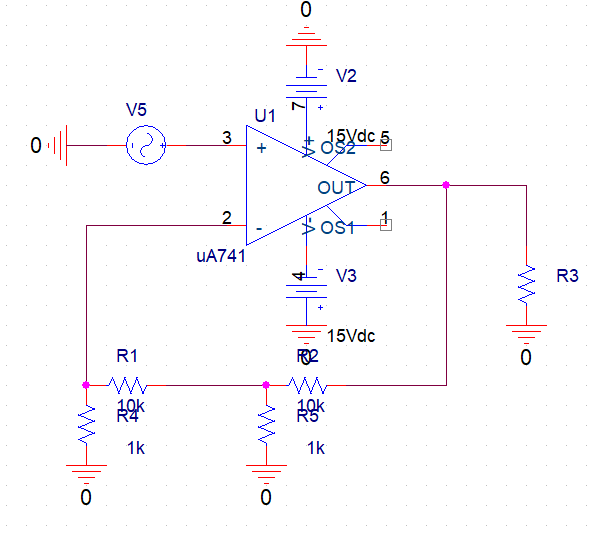
\includegraphics[width=.6\textwidth]{Figures/HW2-6.png}
      \caption{Schematic for Simulation}
      \label{fig:3}
    \end{figure}

    \begin{enumerate}

      \item See plot in Figure \ref{fig:3} below:

        \begin{figure}[H]
          \centering
          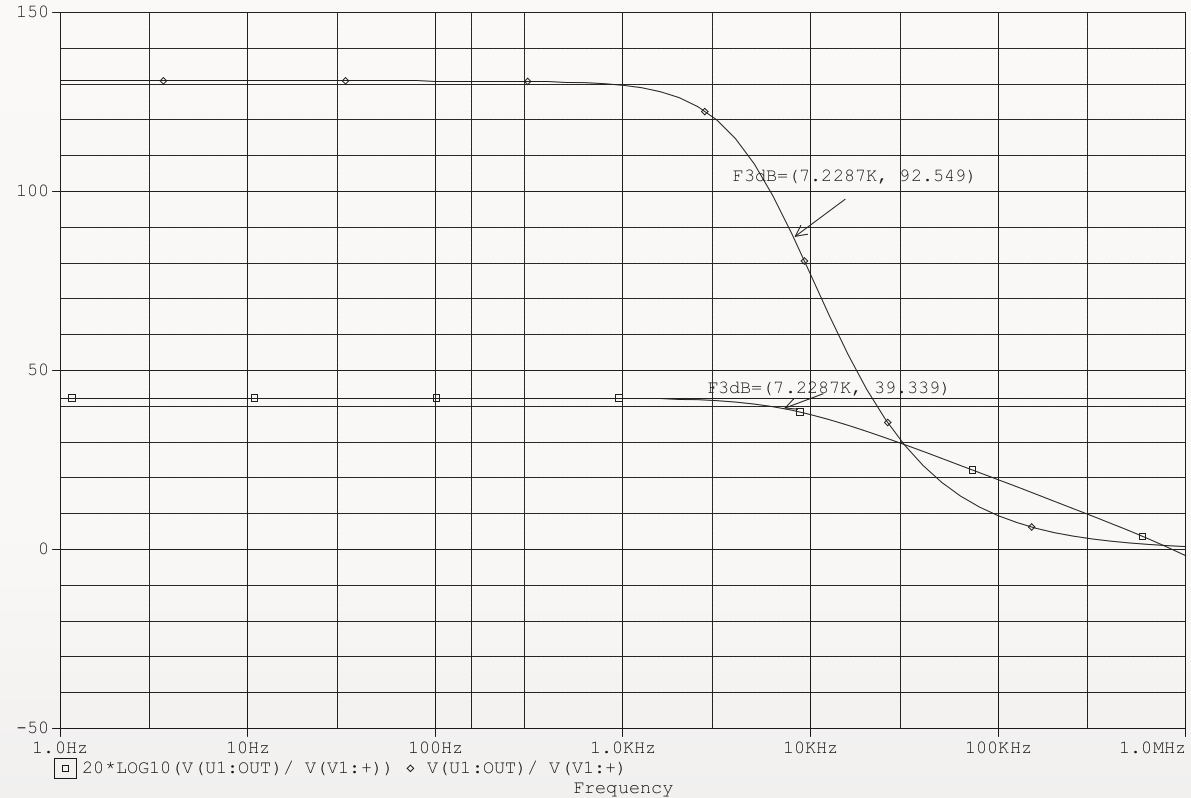
\includegraphics[width=.8\textwidth]{Figures/HW2-6a.png}
          \caption{AC Gain (dB and Magnitude) vs. Frequency}
          \label{fig:4}
        \end{figure}

        Note: the critical frequency is, approximately, $7.2[\si{\kilo\hertz}]$

      \item Note: from this point onwards, the output voltage, $V_o$, uses axis 1, while the input, $V_i$, uses axis 2. See plot in Figure \ref{fig:5} below:

        \begin{figure}[H]
          \centering
          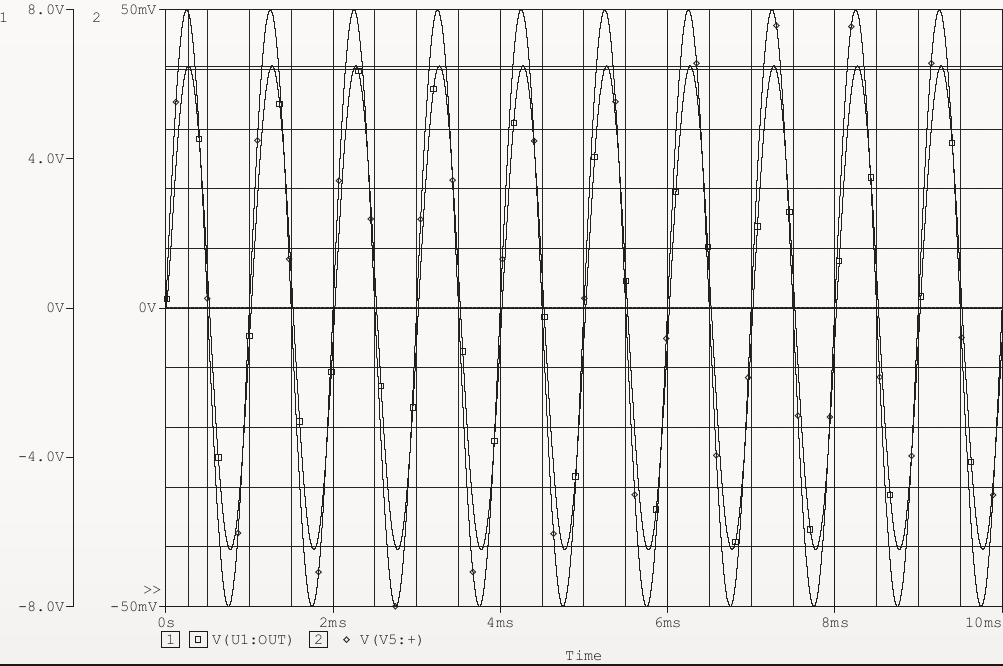
\includegraphics[width=.8\textwidth]{Figures/HW2-6b.png}
          \caption{$V_o$ and $V_i$ vs. Time ($V_i=.05[\si{\volt}]\text{ at }1[\si{\kilo\hertz}])}
          \label{fig:5}
        \end{figure}

        We may notice that the phases are almost identical; however, the magnitude is significantly different. While the input is at the expected $50[\si{\milli\volt}]$, the output is approximately $6.5[\si{\volt}]$ in amplitude. Thus, we can calculate the gain as:

        $$\boxed{A=\frac{6.5}{50\cdot10^{-3}}=130\left[ \frac{\si{\volt}}{\si{\volt}} \right]}$$

      \item See plot in Figure \ref{fig:6} below:

        \begin{figure}[H]
          \centering
          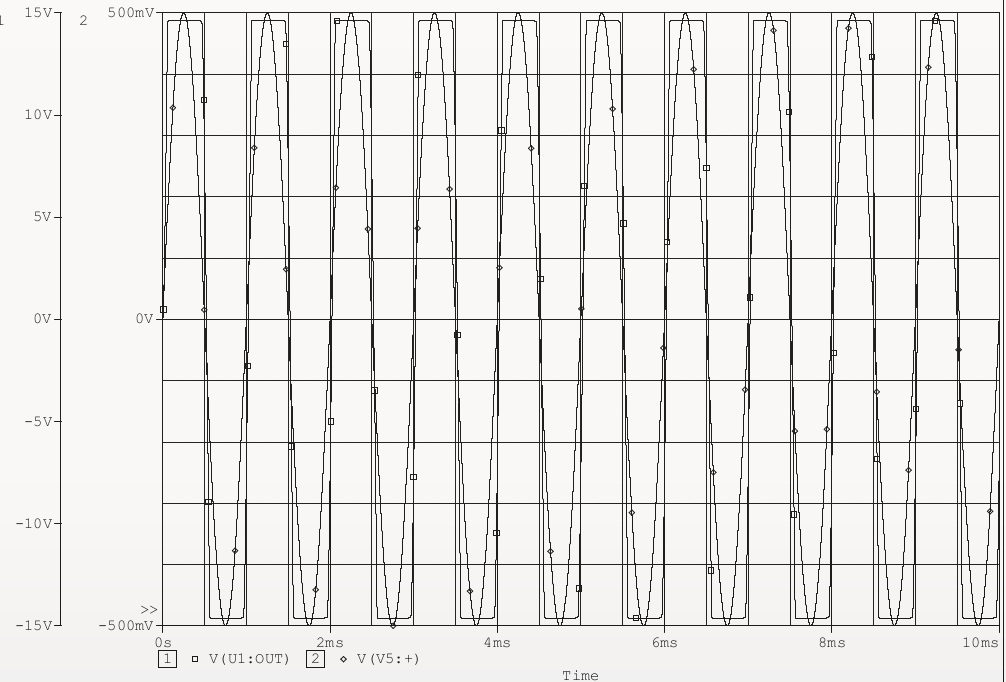
\includegraphics[width=.8\textwidth]{Figures/HW2-6c.png}
          \caption{$V_o$ and $V_i$ vs. Time ($V_i=.5[\si{\volt}]\text{ at }1[\si{\kilo\hertz}])}
          \label{fig:6}
        \end{figure}

        For this plot, we see that, as the output approaches a magnitude of $15[\si{\volt}]$, it begins to form a square wave. This is to be expected, as a $15[\si{\volt}]$ output would saturate the op-amp due to being equivalent to the op-amp DC power supplies. Thus, the output is unable to extend beyond this magnitude, forming the square wave, as would be expected.

      \item See plot in Figure \ref{fig:7} below:

        \begin{figure}[H]
          \centering
          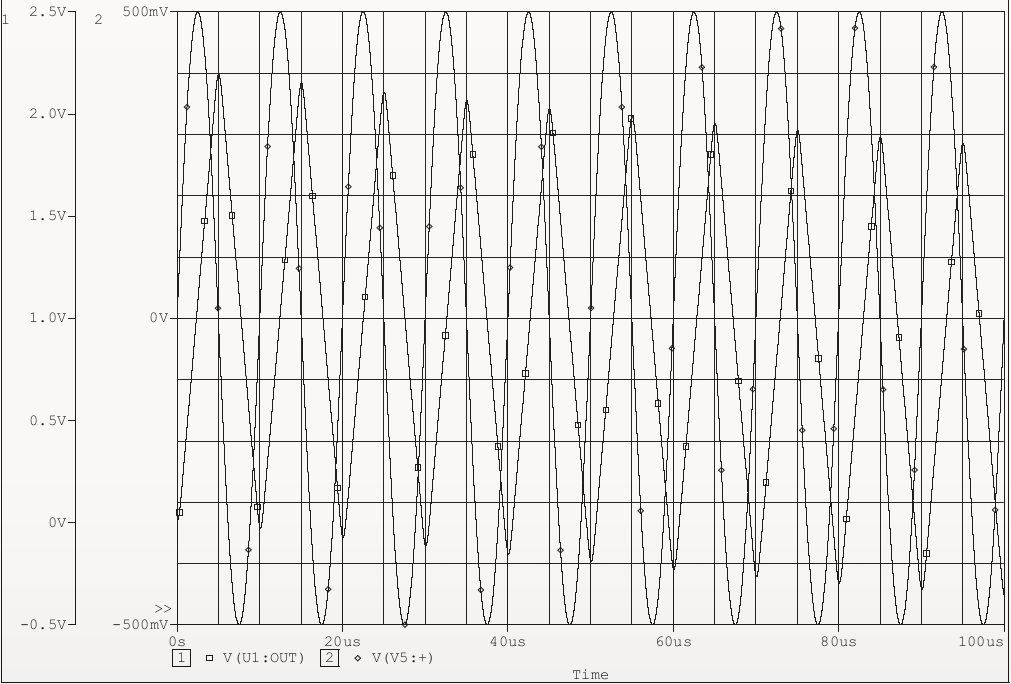
\includegraphics[width=.8\textwidth]{Figures/HW2-6d.png}
          \caption{$V_o$ and $V_i$ vs. Time ($V_i=.5[\si{\volt}]\text{ at }100[\si{\kilo\hertz}])}
          \label{fig:7}
        \end{figure}

        We see that the output begins forming a triangle wave, instead of a sinusoid. Furthermore, the amplitude of the resulting triangle wave is less than would be expected for the gain. The former may be attributed to the slew rate of the op-amp, which, evidently, is less than the input frequency. As a result, the internal capacitors of the op-amp are unable to adjust to the oscillating voltage quickly enough, thus forming a triangle wave. The latter may be attributed to the fact that, as exemplified in Figure \ref{fig:4}, the critical frequency (3dB frequency) occurs at $7.2[\si{\kilo\hertz}]$, which would mean that, at $100[\si{\kilo\hertz}]$, the op-amp would not output a gain that would be nearly as high as expected.

      \item See plot in Figure \ref{fig:8} below:

        \begin{figure}[H]
          \centering
          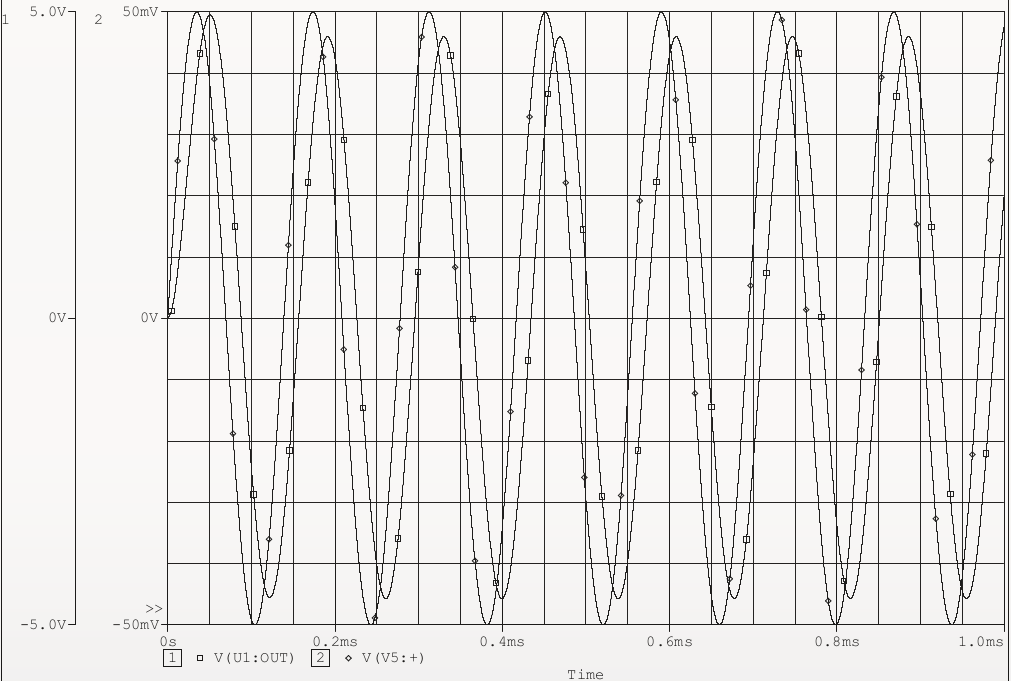
\includegraphics[width=.8\textwidth]{Figures/HW2-6e.png}
          \caption{$V_o$ and $V_i$ vs. Time ($V_i=.05[\si{\volt}]\text{ at }7.2[\si{\kilo\hertz}])}
          \label{fig:8}
        \end{figure}

        In the figure, we see that, at a frequency of $7.2[\si{\kilo\hertz}]$, the op-amp does not output a gain that is as high as at a frequency of $1[\si{\kilo\hertz}]$. This is due to the fact that, as shown in Figure \ref{fig:4}, the critical frequency is at, approximately, $7.2[\si{\kilo\hertz}]$. Looking at Figure \ref{fig:4}, we would expect that the gain would be around $92.5[\si{\volt}/\si{\volt}]$, as demarcated by the $F_{3\text{dB}}$ point. Calculating per the Figure \ref{fig:8}, we get:

        $$\boxed{A=\frac{4.59}{50\cdot10^{-3}}=91.8\left[ \frac{\si{\volt}}{\si{\volt}} \right]}$$

        This value is approximately the expected value.

    \end{enumerate}

\end{enumerate}

\end{document}

